\chapter{Аналитический раздел}
\label{cha:analysis}

%Может лучше убрать эту пасту из вывода?
В данном разделе
описаны понятия активности пользователей и шаблонов поведения пользователей,
проведен обзор и классификация существующих методов анализа активности пользователей,
выбраны критерии для их оценки, проведено сравнение и формализована задача в виде IDEF0-диаграммы.

\section{Активность пользователей}

Тестирование удобства использования программного обеспечения обычно состоит из двух этапов. Первый этап заключается в сборе данных о действиях, совершаемых пользователями посредством взаимодействия с графическим интерфейсом программы (движение курсора мыши, нажатие клавиш мыши, нажатие клавиш клавиатуры и т.д.), и характеристиках действий (координаты курсора, частота нажатия, используемые клавиши и т.д.). Такие данные обозначаются устоявшимся термином «активность пользователей». Второй этап – анализ этих данных экспертом с целью выявления проблем связанных с удобством использования, что является трудоемкой задачей. Поэтому, встает вопрос о хотя бы частичной автоматизации этого этапа, для чего требуется наличие соответствующих моделей и алгоритмов.

\subsection{Шаблоны поведения пользователя}
По мнению многих исследователей (например, авторов \cite{1,4,5,6}), индикатором проблем удобства использования может являться наличие часто повторяемых одинаковых последовательностей действий. Они могут означать, что пользователь пытается достичь цели и каждый раз терпит неудачу. Например, пользователь пытается взаимодействовать с изображением, которое он принял за кнопку \cite{1}, или пользователь нажимает кнопку и каждый раз получает ошибку.

В работе \cite{4} выделен ряд шаблонов, связанных с выполнением пользователем поставленных задач, например, шаблон «Отмена действия», когда пользователь отменяет действие сразу после его выполнения, или шаблон «Повторение действий», когда пользователь часто повторяет простые действия (клики мыши или нажатие клавиш). Наличие второго шаблона может означать недостаточную отзывчивость интерфейса, которая ошибочно приводит пользователя к мысли, что система не распознает его действие.

Отдельные исследователи предлагают отслеживать более простые индикаторы: количество вызовов онлайн-справки, количество действий отмены, частое открытие-закрытие выпадающих списков, нажатие одной и той же кнопки более одного раза и т.д. \cite{5}. Другие исследователи основываются на обнаружении проблем поиска информации пользователем в процессе просмотра веб-сайта \cite{6}. Например, выделяется шаблон вертикального или горизонтального перемещения курсора мыши. В процессе визуального поиска на странице пользователь обычно перемещает курсор вслед за элементами, а значит, тратит много времени на поиск элемента.

Перечисленные методы поиска шаблонов поведения пользователей имеют много общего с задачей поиска последовательных шаблонов из области интеллектуального анализа данных [7]. В большинстве случаев все шаблоны являются последовательными, варьируются лишь анализируемые события. Однако данные активности пользователей почти всегда представляют собой не короткие транзакции, а большие наборы действий, которые в большинстве случаев невозможно корректно разделить на поднаборы \cite{2,3}.

Поиск последовательных шаблонов давно и активно применяется в области торговли [8]. Поиск наиболее частых наборов позволяет получать
информацию о том, через какой промежуток времени после покупки товара «А» человек наиболее склонен купить товар «Б» или в какой последовательности приобретаются товары. Получаемые закономерности в действиях покупателей можно использовать для персонализации клиентов, стимулирования продаж определенных товаров, управления запасами [8]. Это позволяет, с одной стороны, увеличить продажи, с другой – предложить клиентам товар, который, скорее всего, будет им интересен, а значит, минимизировать их временные затраты на поиск.

%При проектировании пользовательского интерфейса в соответствии со стандартами ГОСТ-2880690 и ISO 9241-11:1998 аналогичным образом требуется максимизировать результативность (точность и полноту достижения пользователем поставленных целей, успешность выполнения промежуточных задач) и эффективность (отношение израсходованных ресурсов к точности и полноте, с которой пользователи достигают поставленных целей).

Как уже отмечалось, одной из возможных причин появления регулярно повторяющихся шаблонов в данных активности пользователей является
наличие ошибок или затруднений при взаимодействии с интерфейсом. В этом случае может наблюдаться снижение и результативности, и эффективности пользователей. Следовательно, уменьшение числа подобных шаблонов снижает риск возникновения ошибок.

Другой возможной причиной наличия повторяющихся шаблонов в данных активности пользователей является потребность выполнения одних и
тех же повторяющихся цепочек действий для выполнения поставленных задач. Закономерно, что автоматизация промежуточных действий уменьшает затраты ресурсов. Следовательно, чем меньше пользователь совершает однотипных цепочек действий, тем меньше он затрачивает ресурсов, а значит, тем эффективнее взаимодействие.

Конечно, при этом отмечается, что повторяющиеся шаблоны могут быть образованы из-за повторяющихся задач, которые либо невозможно или
нецелесообразно автоматизировать, либо являются нормальным корректным поведением \cite{1}. Поэтому требуется понимание семантики шаблонов и конкретных действий.

\section{Существующие решения}

\subsection{Математическая модель пользовательской активности ПО}
В статье \cite{mat_model} предлагается математическая модель активности пользователей ПО, основанная на теории последовательных шаблонов для предметной области оценки удобства использования. Данный способ совмещает анализ временных характеристик с вычислением уровней поддержки последовательных шаблонов.

Модель состоит из следующих элементов:
\begin{itemize}
	\item[---] множество событий с атрибутами;
	\item[---] множество классов событий;
	\item[---] функция классификации событий;
	\item[---] множество сессий до классификации;
	\item[---] множество сессий после классификации и фильтрации;
	\item[---] множество последовательных шаблонов;
	\item[---] множество значений поддержки последовательных шаблонов;
	\item[---] функция преобразования класса событий в затрачиваемое время.
\end{itemize}

%В качестве функции преобразовния класса событий в затрачиваемое время можно использовать метод оценки эффективности интерфейса – GOMS (Goals, Operators, Methods, Selection Rules – Цели, Операторы, Методы, Правила выбора соответственно), который включает в себя модель Keystroke-level Model (KLM) \cite{11}.

Данная модель может найти применение при оценке удобства использования пользовательских интерфейсов и для решения задач повышения эффективности взаимодействия пользователей с ПО.

Имея значения поддержки и затрачиваемого времени для каждого шаблона, эксперт может сконцентрироваться на наиболее значимых из них
для процесса работы пользователей с ПО в целом. Набор шаблонов при этом будет зависеть от целей проводимого анализа.

Далее эксперт может выдвинуть гипотезы о необходимых изменениях в пользовательском интерфейсе для повышения эффективности взаимодействия пользователей с ПО. При принятии решений эксперту необходимо учитывать множество различных факторов: особенности ПО, психологические факторы использования ПО и особенности пользователей.

Изменение пользовательского интерфейса повлечет изменение множеств событий, сессий и последовательных шаблонов, так как изменится
последовательность действий, необходимых для достижения пользователями поставленных целей.

Таким образом, можно утверждать, что задачей эксперта становится переход от текущей модели активности пользователей к новой, с иным составом сессий и шаблонов, следовательно, и иными значениями поддержки шаблонов и затратами времени пользователей.

После внесения изменений в программный интерфейс возможны повторный сбор и анализ данных активности пользователей, что может подтвердить либо опровергнуть выдвинутую ранее гипотезу.

Недостатком данной модели является использование заранее предопределенных шаблонов.

\subsection{Алгоритм получения ассоциативных правил Apriori}
Базовым алгоритмом, применяемым для получения ассоциативных правил, является алгоритм Apriori \cite{34}, автором которого является Ракеш Агравал (Rakesh Agrawal). Алгоритм Apriori использует стратегию поиска в ширину и осуществляет его снизу-вверх, последовательно перебирая кандидатов.
В алгоритме используются две структуры данных: $C_i$ — для хранения множества кандидатов в частые множества признаков длины $i$ и $F_i$ — для хранения частых множеств признаков длины $i$. Каждая структура имеет два поля — itemset, сохраняющее множество признаков, и support, которое хранит величину поддержки этого множества признаков. Ниже представлена формальная запись алгоритма состоящего из двух частей: самого Apriori и вспомогательной процедуры AprioriGen. 
%(рис. \ref{img:Apriori}).

%\imgsc{H}{0.7}{Apriori}{Алгоритм Apriori, перебор кандидатов шаблонов.}

%\newpage
Apriori$(Context, min\_supp)$. Context - набор данных, min\_supp - минимальная поддержка, $I_F$ -- все частые множества признаков.

\noindent
$C_1 \leftarrow \{1-itemsets\}  \\
i \leftarrow 1 \\
\textbf{while} (C_i \ne 0) \\
\textbf{do}
\begin{cases}
	SupportCount(C_i)\\
	F_i \leftarrow \{f \in C_i | f.support \ge min\_supp\} \text{//F -- частые множества признаков} \\
	C_{i+1} \leftarrow AprioriGen(F_i) \text{//C -- кандидаты} \\
	i++
\end{cases} \\
I_F \leftarrow \cup F_i \\
\textbf{return}(I_F)$

%(рис. \ref{img:AprioriGen}).

\newpage
%\imgsc{H}{0.7}{AprioriGen}{Алгоритм AprioriGen, формирование кандидатов шаблонов.}
AprioriGen$(F_i)$. $F_i$ - частые множества признаков длины $i$, $C_{i+1}$ -- потенциальные кандидаты частых множеств признаков.

\noindent
%insert into $C_{i+1}$ // объединенее \\
%select $p[1],p[2],...,p[i],q[i]$ \\
%from $F_ip, F_iq$ \\
%where $p[1]=q[1],...,p[i-1]=q[i-1],p[i]<q[i]$ \\
%// Получение всевозможных множеств длины i+1 на основе Fi
%$C_{i+1} \leftarrow Union(F_i)$ // объединение \\
%$C_{i+1} \leftarrow \{p \cup q_{k-1} | \forall p \in F_i, q \in F_i: p_1=q_1, p_2=q_2, p_{k-2}=q_{k-2}, p_{k-1}<q_{k-1} \}$ \\
$C_{i+1} \leftarrow \{p \cup q | p, q \in F_i,| p \cap q| = k-2 \}$ \\
\textbf{for each} $c \in C_{i+1}$ // удаление \\
\textbf{do}
$\begin{cases}
	S \leftarrow (i-1)-\text{элементарные подмножества } c\\
	\textbf{for each } s \in S \text{// удаление} \\
	\textbf{do} 
	\begin{cases}
		\textbf{if } (s \notin F_i)\\
		\textbf{then } C_{i+1} \leftarrow C_{i+1} \backslash c
	\end{cases} \\
	\textbf{return} (C_{i+1})
\end{cases}$

Основной особенностью алгоритма можно считать использование свойства антимонотонности, которое гласит, что поддержка любого набора элементов не может превышать минимальной поддержки любого из его подмножеств. Именно благодаря этому свойству перебор не является «жадным» и позволяет обрабатывать большие массивы информации за секунды.

Существуют различные модификации алгоритма Apriori и иные алгоритмы \cite{35}, значительно оптимизированные под определенные ситуации. Можно утверждать, что применение существующего проработанного аппарата теории последовательных шаблонов позволит реализовать поиск неизвестных ранее шаблонов взаимодействия пользователей c интерфейсом программы.
%с информационной системой при меньших временных затратах.

Алгоритмическая сложность данного метода экспоненциальна: $O(|D| \cdot |I| \cdot 2^{|I|})$, где $|D|$ -- количество транзакций в исходном наборе данных, а $|I|$ -- общее число предметов \cite{Data_mining_book}. Но это верно только для худшего случая, если задать минимальный уровень поддержки = 0, что не имеет практического смысла, т.к. интерес представляют ассоциативные правила с высоким уровнем поддержки.

\subsection{Алгоритм GSP}
Алгоритм GSP (англ. Generalized Sequential Pattern, обобщенный секвенциальный паттерн) является модификацией алгоритма AprioriAll, учитывающей ограничения по времени между соседними транзакциями \cite{1_, 32_}.

В случае с алгоритмом GSP требуется учитывать дополнительные условия, чтобы определить, содержит ли последовательность указанную подпоследовательность \cite{gsp}.

Введем такие параметры, как минимальное и максимальное допустимое время между транзакциями ($min\_gap$ и $max\_gap$), а также понятие скользящего окна, размера $win\_size$. Допускается, что элемент последовательности может состоять не из одной, а из нескольких транзакций, если разница во времени между ними меньше, чем размер окна.

Последовательность $d = \langle d_1...d_m \rangle$ содержит последовательность
$s = \langle s_1...s_m \rangle$, если существуют такие целые числа $l_1 ≤ u_1 < l_2 ≤ u_2 < ... < l_n ≤ u_n$, что:

\begin{enumerate}
	\item[---] $s_i$ содержится в объединении $d_k$, где $l_i ≤ k ≤ u_i, 1 ≤ i ≤ n$.
	\item[---] $t_{\text{транзакции}}(d_{l[i]}) - t_{\text{транзакции}} (d_{u[i-1]}) ≤ win\_size, 1 ≤ i ≤ n.$
	\item[---] $min\_gap ≤ t_{\text{транзакции}}(d_{l[i]}) - t_{\text{транзакции}}(d_{u[i-1]}) ≤ max\_gap,$ \newline $2≤i≤n.$
\end{enumerate}

Выполнение алгоритма GSP предусматривает несколько проходов по исходному набору данных. При первом проходе вычисляется поддержка для каждого предмета и из них выделяются частые. Каждый подобный предмет представляет собой одноэлементную последовательность. В начале каждого последующего прохода имеется некоторое число ЧВП (часто встречающихся последовательностей), выявленных на предыдущем шаге алгоритма. Из них будут формироваться более длинные последовательности-кандидаты.

Каждый кандидат представляет собой последовательность, длина которой \textit{на один больше} чем у последовательностей, из которых кандидат был сформирован. Таким образом, число элементов всех кандидатов одинаково. После формирования кандидатов происходит вычисление их поддержки. В конце шага определяется, какие кандидаты являются ЧВП. Найденные ЧВП послужат исходными данными для следующего шага алгоритма. Работа алгоритма завершается тогда, когда не найдено ни одной новой ЧВП в конце очередного шага, или когда невозможно сформировать новых кандидатов.

Таким образом, в работе алгоритма можно выделить следующие основные этапы:

%1. Генерация кандидатов. \\
%\indent 1.1. Объединение. \\
%\indent 1.2. Упрощение. \\
%\indent 2. Подсчет поддержки кандидатов.\\

%нужно ли здесь \item[---] или норм \item[1.]
\begin{enumerate}
	\item[1.] Генерация кандидатов.
	\begin{enumerate}
		\item[1.] Объединение.
		\item[2.] Упрощение.
	\end{enumerate}
	\item[2.] Подсчет поддержки кандидатов.
\end{enumerate}

Рассмотрим эти операции более подробно.

\textbf{Этап 1. Генерация кандидатов.} Пусть $L_k$ содержит все частые $k$-последовательности, а $C_k$ – множество кандидатов из $k$-последовательностей. В начале каждого шага имеем $L_{k-1}$ – набор из $(k-1)$ ЧВП. На их основе необходимо построить набор всех $k$ ЧВП.

Введем понятие \textit{смежной подпоследовательности}.

При наличии последовательности $s = \langle s1, s2..., sn \rangle$ и подпоследовательности $c$, $c$ будет являться \textit{смежной последовательностью} $s$, если соблюдается одно из условий:
\begin{itemize}
	\item[---] $c$ получается из $s$ при удалении предмета из первого $\{s_1\}$ или последнего $\{s_n\}$ предметного множества;
	\item[---] $c$ получается из $s$ при удалении одного предмета из предметного множества $s_i$, если в его составе не менее двух предметов;
	\item[---] $c$ – смежная подпоследовательность $c'$, где $c'$ – смежная подпоследовательность $s$.
\end{itemize}

Например, дана последовательность $s = \langle\{1,2\},\{3,4\},\{5\},\{6\}\rangle$. Последовательности $\langle\{2\},\{3,4\},\{5\}\rangle$, $\langle\{1,2\},\{3\},\{5\},\{6\}\rangle$ и $\langle\{3\},\{5\}\rangle$ являются смежными подпоследовательностями $s$, а последовательности $\langle\{1,2\},\{3,4\},\{6\}\rangle$ и $\langle\{1\},\{5\},\{6\}\rangle$ таковыми не являются.

Если некоторая последовательность содержит последовательность $s$, то она также содержит и все смежные подпоследовательности $s$.

Генерация кандидатов происходит в два этапа.
%(условно назовем эти этапы функцией $candidate\_gen\_SPM()$).

\textbf{Этап 1.1. Объединение} (англ. \textit{join}). Создаем последовательности-кандидаты путем объединения двух последовательностей $L_{k−1}$ и $L_{k−1}$. Последовательность $s_1$ объединяется с $s_2$, если подпоследовательность, образующаяся путем удаления первого предмета из $s_1$, будет та же, что и в случае удаления последнего предмета из $s_2$. Объединение последовательностей происходит путем добавления к $s_1$ соответствующего предмета из последнего предметного множества $s_2$. Причем возможны два варианта:
\begin{itemize}
	\item[---] если последний предмет из $s_2$ составлял одноэлементное предметное множество, то при объединении он будет добавлен к $s_1$ как новое предметное множество;
	\item[---] в противном случае, он будет включен в последнее предметное множество $s_1$ как его элемент.
\end{itemize}

При объединении $L_1$ c $L_1$ нужно добавить предмет к $s_2$ как отдельное предметное множество, а также в качестве дополнительного предмета в предметное множество последовательности $s_1$. Так, объединение $\langle\{x\}\rangle$ с $\langle\{y\}\rangle$ дадут как $\langle\{x, y\}\rangle$, так и $\langle\{x\},\{y\}\rangle$. Причем $x$ и $y$ упорядочены.

\textbf{Этап 1.2. Упрощение} (англ. \textit{prune}). Удаляем последовательности кандидаты, которые содержат смежные $(k-1)$-последовательности, чья поддержка меньше минимально допустимой.

\textbf{Этап 2. Подсчет поддержки кандидатов.} Сканируя набор последовательностей, обрабатываем их по очереди. Для тех кандидатов, которые содержатся в обрабатываемой последовательности, увеличиваем значение поддержки на единицу.	

%Добавить?
%Недостатками подобных алгоритмов, существенно снижающими вычислительную эффективность обработки данных, являются:
%\begin{itemize}
%	\item[---] большое количество обращений к базе данных, соответствующее длине максимального кандидата-последовательности;
%	\item[---] большое число генерируемых кандидатов-последовательностей.
%\end{itemize}

Алгоритмическая сложность данного метода экспоненциальна: $O(|I|^l)$, где $|I|$ -- общее число предметов, а $l$ -- длина наибольшей часто встречающейся последовательности \cite{Data_mining_book}.

\subsection{Метод оценки эффективности интерфейса GOMS}
Метод GOMS (сокращение от Goals, Operators, Methods and Selection Rules -- Цели, Операторы, Методы и Правила выбора) -- это семейство методов, позволяющих провести моделирование выполнения той или иной задачи пользователем и на основе такой модели оценить качество интерфейса.

Идея метода заключается в разбиении взаимодействия пользователя с интерфейсом на атомарные физические и когнитивные действия. Обладая знаниями о метриках каждой из таких составляющих, можно делать заключение об эффективности взаимодействия в целом: оценка
эффективности интерфейса сводится к разбиению типовых задач на элементарные действия и сложению метрик каждого из них.

Метод GOMS включает в себя модель Keystroke-level Model (KLM) \cite{11}, которая выделяет следующие элементарные задачи и длительность каждой из них (рассчитанные на основе усредненных данных лабораторных испытаний):

\begin{itemize}
	\item[---] K – нажатие на клавишу в зависимости от уровня владения клавиатурой: профессиональный	наборщик – 0.08 сек., эксперт – 0.12 сек., частая работа с текстом – 0.20 сек., продвинутый пользователь – 0.28 сек., неуверенный пользователь – 0.5 сек., не знакомый с клавиатурой – 1.2 сек.;
	\item[---] P – указание курсором мыши на объект – 1.1 сек.;
	\item[---] B – нажатие или отпускание мыши – 0.1 сек.;
	\item[---] M – умственная подготовка, выбор действия – 1.2 сек.;
	\item[---] H – перемещение руки в исходное положение на клавиатуре – 0.4 сек;
	\item[---] R – ожидание ответа системы, зависящее от	времени выполнения системой запрошенной операции.
\end{itemize}

Оценка времени на решение задачи сводится к сложению продолжительностей каждой из простейших составляющих. Например, задача, состоящая из классов (P, P, B), потребует для завершения 2.3 сек. (1.1 сек. + 1.1 сек. + 0.1 сек.).

%\newpage
\subsection{Классификация} %Убрать?
Рассмотрев вышеописанные методы анализа пользовательской активности, можно их разделить на следующие категории:
\begin{itemize}
	%	\item поиск последовательных шаблонов; %поиск ассоциативных правил;
	\item[---] поиск ассоциативных правил (Apriori);
	\item[---] поиск последовательных шаблонов (GSP);
	\item[---] сбор и анализ временных характеристик выполнения пользователем действий и промежутков между ними (GOMS);
	\item[---] вычисление уровней поддержки шаблонов поведения пользователя (Математическая модель пользовательской активности ПО).
\end{itemize}

%Вычисление уровней поддержки шаблонов поведения пользователя позволяет ранжировать их по степени приоритета для детального анализа.
%Методы поиска ассоциативных правил и последовательных шаблонов позволяют найти новые (неизвестные ранее) шаблоны взаимодействия пользователей с программным обеспечением.
%А анализ временных характеристик, позволяет оценить эффективность взаимодействия пользователя с интерфейсом.


\section{Сравнение}

В таблице \ref{tab} приведено сравнение рассмотренных методов.

\begin{table}[H]
	\begin{center}
		\caption{Сравнение рассмотренных методов}
		\label{tab}
		""\newline
		\begin{tabular}{ | c | c | c | c | }
			\hline
			Метод & \specialcell{Требование к\\ входным данным}  & \specialcell{Учет\\времени \\транз-ий} & \specialcell{Сложность\\алгоритма} \\ \hline
			
			\specialcell{Мат. модель\\пользов.\\актив. ПО} & \specialcell{Множество событий,\\функция классификации\\событий, множество\\сессий, множество\\последовательных\\шаблонов} & Нет & \specialcell{$O(n \cdot m)$, где $n$ --\\кол-во шаблонов,\\$m$ -- кол-во сессий} \\ \hline
			
			\specialcell{Apriori} & \specialcell{Транзакции с набором\\элементов и\\минимальный уровень\\поддержки} & Нет & \specialcell{$O(|D| \cdot |I| \cdot 2^{|I|})$,\\где $|D|$ -- кол-во\\транзакций,\\$|I|$ -- общее число\\предметов} \\ \hline
			
			\specialcell{GSP} & \specialcell{База данных с полями:\\id последовательности,\\id и время транзакции,\\набор элементов\\и минимальный\\уровень поддержки} & Да & \specialcell{$O(|I|^l)$, где $|I|$ --\\общее число\\предметов,\\$l$ -- длина\\наибольшей ЧВП} \\ \hline
			
			\specialcell{GOMS} & \specialcell{Последовательность\\действий} & Нет & \specialcell{$O(n)$, где n --\\число действий\\в послед-ти} \\ \hline
		\end{tabular}
	\end{center}
\end{table}

%Убрать вместе с классификацией?
Вычисление уровней поддержки шаблонов поведения пользователя позволяет ранжировать их по степени приоритета для детального анализа.
Методы поиска ассоциативных правил и последовательных шаблонов позволяют найти новые (неизвестные ранее) шаблоны взаимодействия пользователей с программным обеспечением.
А анализ временных характеристик, позволяет оценить эффективность взаимодействия пользователя с интерфейсом.

%Изменить?
\section{Формализованная постановка задачи}
Поскольку
%в данной работе стоит задача реализации метода анализа активности пользователей САПР с использованием поиска последовательных шаблонов, а в подобных программах
активность пользователей представляет собой последовательность действий и их характеристик, производящихся в определенный момент времени, то за основу был выбран алгоритм GSP, т.к. он учитывает время совершения транзакций.

Для выполнения дальнейшей работы необходимо формализовать задачу анализа активности пользователей САПР. Поставленная задача представлена в нотации IDEF0 на рисунке \ref{idef0}. На вход программе подаются информация о выполненных командах (логи), минимальный уровень поддержки, минимальный и максимальный разрывы между командами. Используя методы поиска последовательных шаблонов система определяет часто встречающиеся последовательности команд.

\begin{figure}[h!]
	\centering
	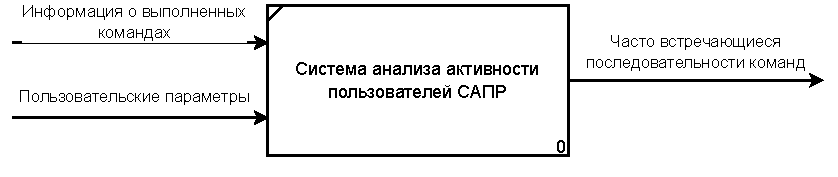
\includegraphics[width=1.0\textwidth]{inc/img/IDEF0.drawio.pdf}
	\caption{IDEF0-диаграмма первого уровня}
	\label{idef0}
\end{figure}

\section*{Вывод из аналитического раздела}

В данном разделе был проведен обзор существующих методов анализа пользовательской активности, сформулированы критерии для их оценки, проведено сравнение рассмотренных методов и формализована задача в виде IDEF-0 диаграммы.